\section{Curves}

\subsection{Kurve in der Ebene}

\textbf{Explizite Darstellung} \\
$\gamma : [a,b] \rightarrow \mathbb{R} , x \mapsto y = f(x)$ \\
\textit{Kreis: \\oberer Halbkreis $\sqrt{r^2 - x^2}$ \\ unterer Halbkreis $\sqrt{r^2 - x^2}$} \\
\\
\textit{(Implizite Darstellung nach $y$ auflösen -> Explizite Darstellung)}\\
\\
\textbf{Implizite Darstellung} \\
$F(x,y) = 0$ \\
\textit{Kreis mir radius $r$ und Zentrum $(0,0)$:} \\
\textit{$x^2 + y^2 - r^2 = 0$}
\\
\textbf{Parameterdarstellung} \\
$\gamma : [a,b] \rightarrow \mathbb{R}^2,t \mapsto X(t) = \begin{bmatrix} x_1(t) \\ x_2(t) \end{bmatrix}$ \\
\textit{Punkte miteinander verbunden, einzeln angegeben} \\
\textit{Kreis: $\begin{bmatrix} r \cos t \\ r \sin t \end{bmatrix}$}\\
\\
\textit{-> einzelne Funktionen für $x$ \& $y$}\\

\textit{Beachte, Parameterdarstellung ist nicht eindeutig;}\\
\textit{$\gamma : [0,\pi] \rightarrow \mathbb{R}^2,t \mapsto X(t) =
\begin{bmatrix}
    r \cos(2t) \\ r \cos(2t)
\end{bmatrix}$, Kreis doppelt so schnell durchlaufen ($2t$)}

\textit{$\gamma : [0,\pi] \rightarrow \mathbb{R}^2,t \mapsto X(t) =
\begin{bmatrix}
    r \cos(2\pi t) \\ r \cos(2\pi t)
\end{bmatrix}$, Kreis durchlaufen in einer Zeiteinheit 1 ($2\pi t$)}

\subsection{Kurve im Raum}
\textit{Parameterdarstellung mit 3 Komponenten}

$\gamma : [a,b] \rightarrow \mathbb{R}^3,t \mapsto X(t) =
\begin{bmatrix}
    x_1(t) \\
    x_2(t) \\
    x_3(t)
\end{bmatrix}$

\subsection{Spirale entlang des Zylinders}


\begin{tabular}{cl}
    \multirow{8}{*}{
        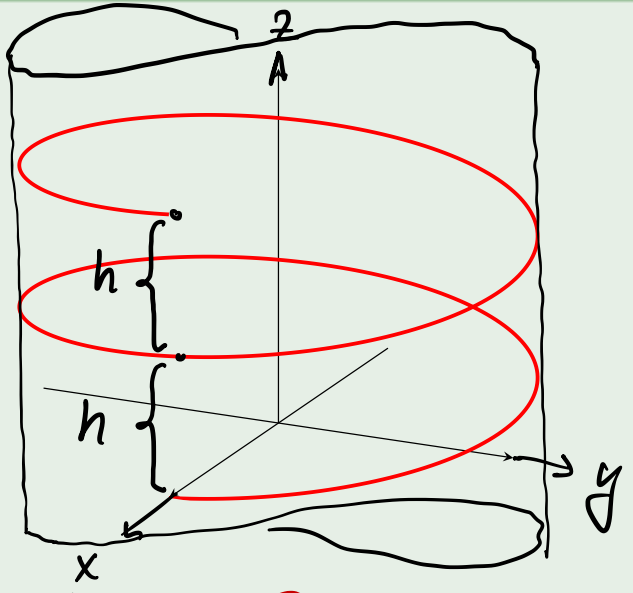
\includegraphics[width=0.18\textwidth]{assets/curves-spiral-following-cylinder.png}
    } & $x^2 + y^2 = r^2$ \\
    & \\
    & $\gamma : [0, 4\pi] \rightarrow \mathbb{R}^3,$ \\
    & $t \mapsto X(t) = \begin{bmatrix}
        r \cos t \\ r sin t \\ ht / (2\pi)
    \end{bmatrix}$ \\
    & \textit{Grundriss ergibt Kreis, Höhe Linear} \\
    & \\
\end{tabular}

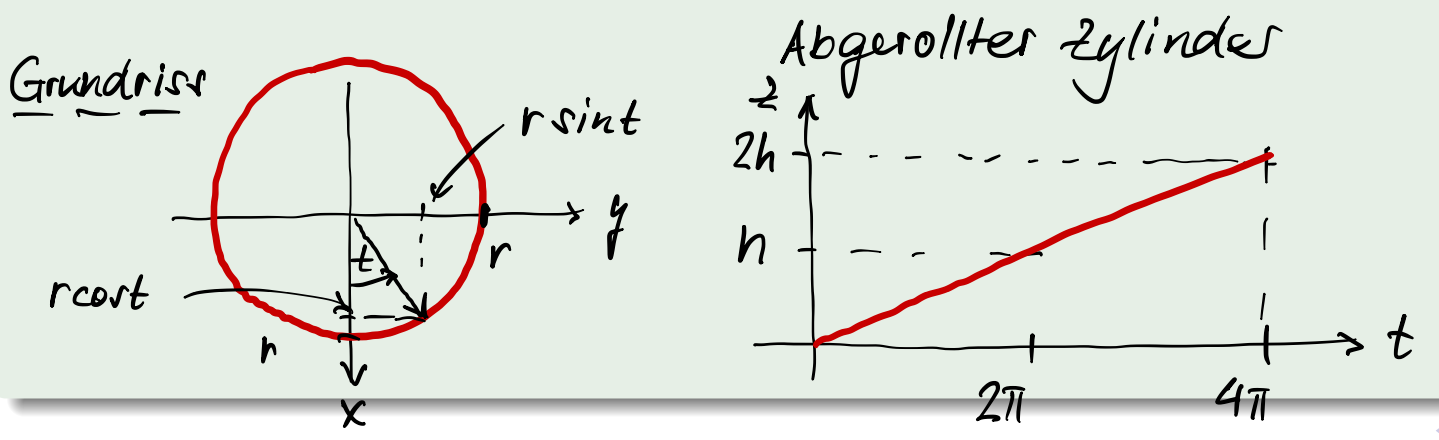
\includegraphics[width=0.5\textwidth]{assets/curves-spiral-following-cylinder-sol.png}

\subsection{Splines Übersicht (Interpolation versus Approximation)}
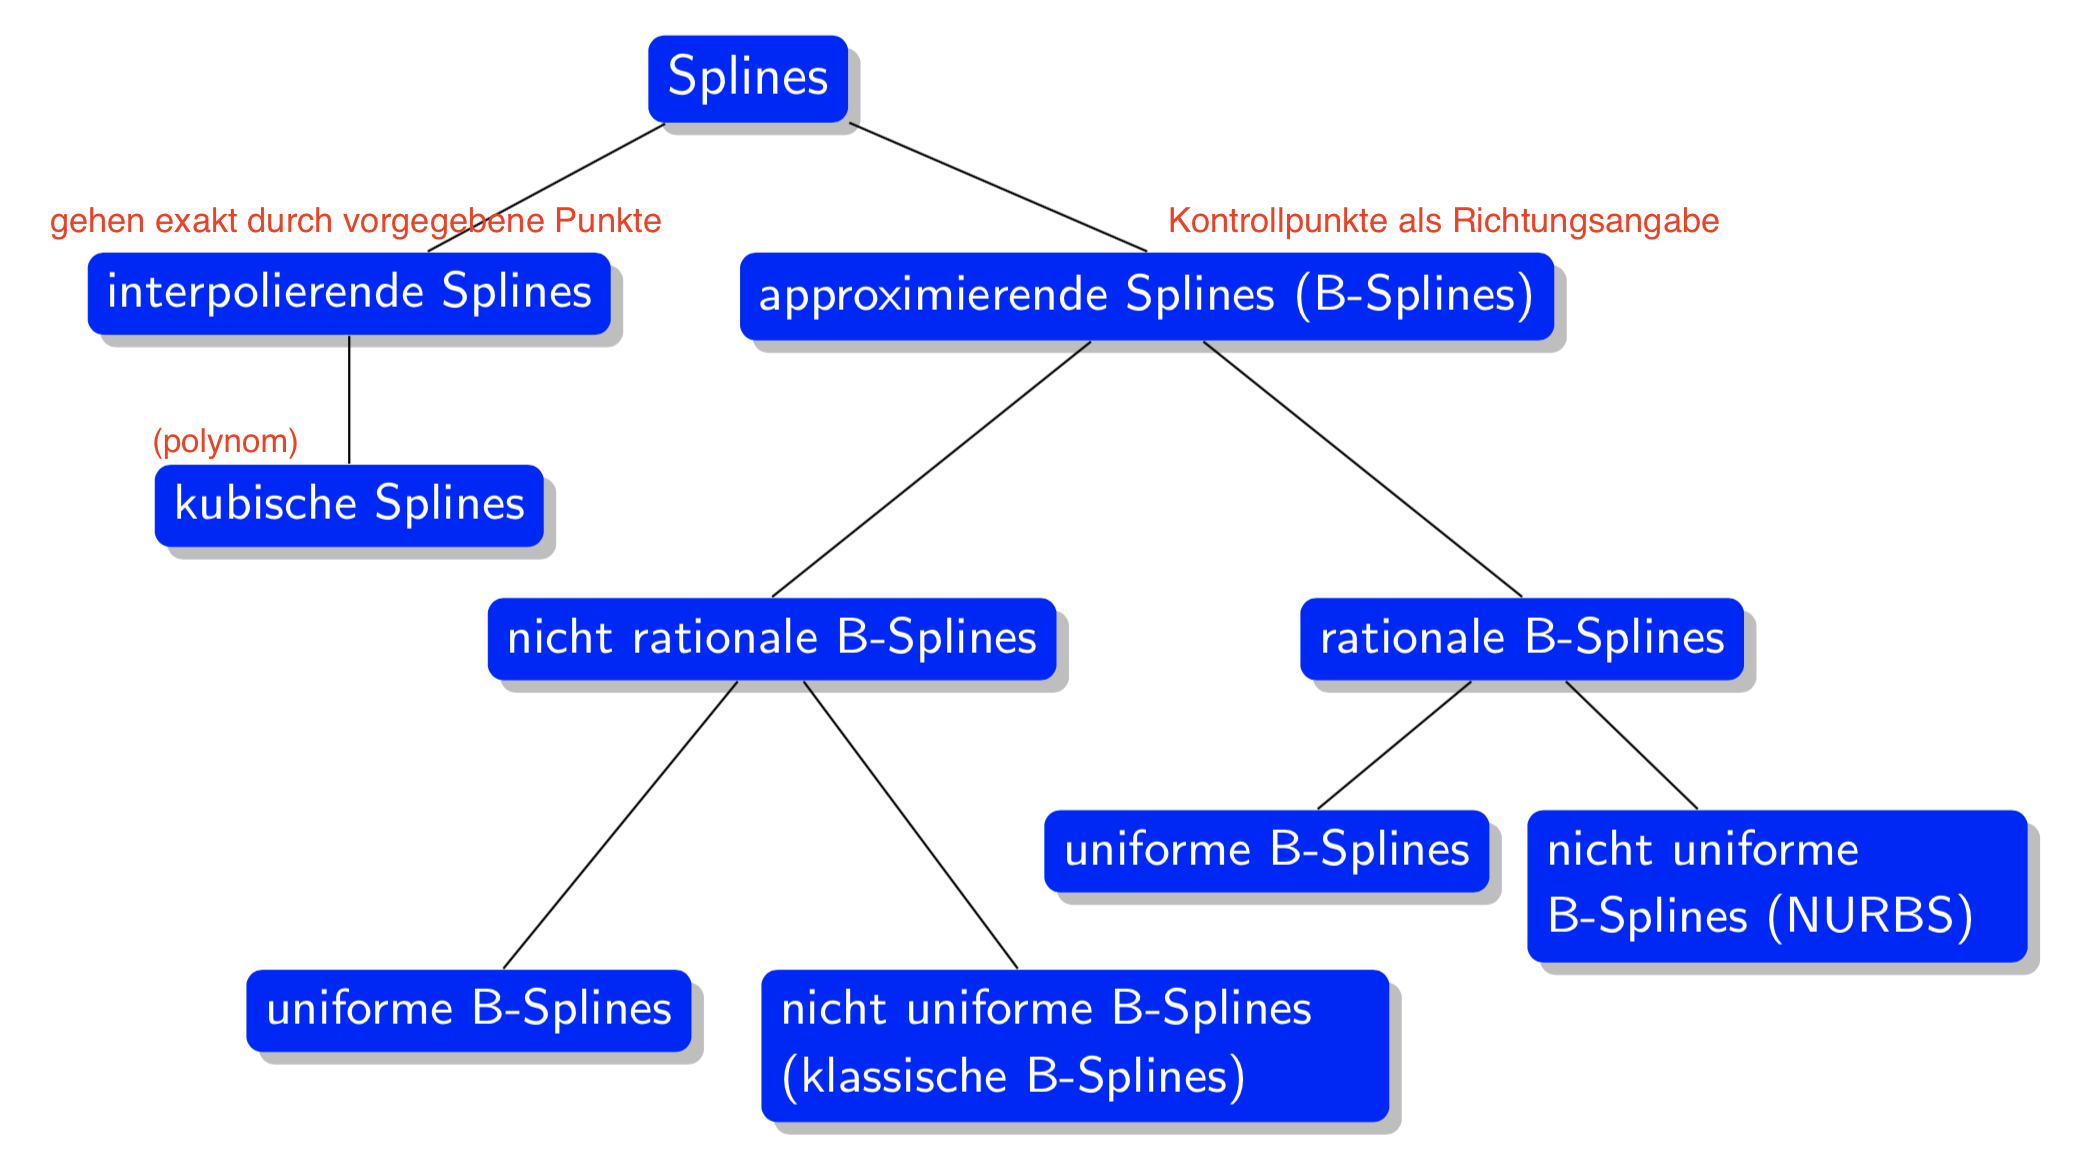
\includegraphics[width=0.5\textwidth]{assets/InterpolationVSApproximation.png}


\subsection{Methode unbestimmte Koeffizienten (Interpolation)}
$P_3(x) = c_0 + c_1x + c_2x^2 + c_3x^3$ \\
\\
\textit{Auflösen durch einfügen von $P_0(x_0, y_0)$, $P_1(x_1, y_1)$, $P_2(x_2, y_2)$, ..}
\\
    $\begin{bmatrix}
    1 & x_0 & x_0^2 & x_0^3 \\
    1 & x_1 & x_1^2 & x_1^3 \\
    1 & x_2 & x_2^2 & x_2^3 \\
    1 & x_3 & x_3^2 & x_3^3 \\
\end{bmatrix}
\begin{bmatrix}
    c_0 \\
    c_1 \\
    c_2 \\
    c_3
\end{bmatrix} =
\begin{bmatrix}
    y_0 \\
    y_1 \\
    y_2 \\
    y_3
\end{bmatrix}$ \\
\\
\textit{$c_0 = c_1 = c_2 = c_3 = 1$}

\subsection{Lagrange Methode (Interpolation)}

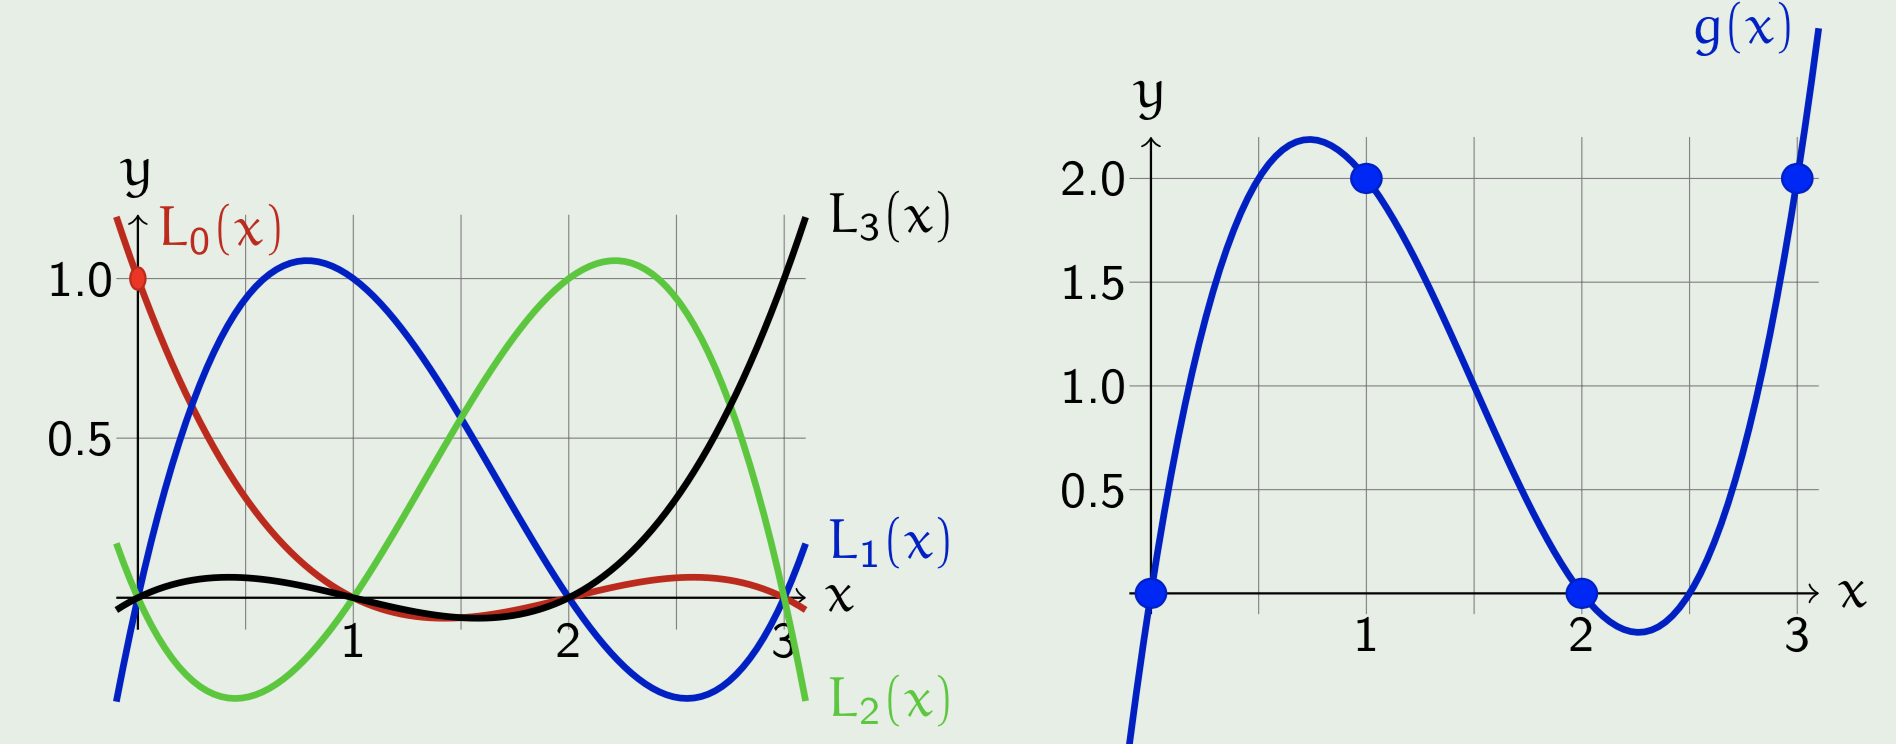
\includegraphics[width=0.5\textwidth]{assets/Lagrange1.png}
Polynome 3. Grades, welche an allen Stützstellen Null sind ausser an einer, wo der Wert Eins (1) sein soll:
$L_0(x) = \frac{(x-x_1)(x-x_2)(x-x_3)}{(x_0-x_1)(x_0-x_2)(x_0-x_3)}$ \\
$L_1(x) = \frac{(x-x_0)(x-x_2)(x-x_3)}{(x_1-x_0)(x_1-x_2)(x_1-x_3)}$ \\
$L_2(x) = \frac{(x-x_0)(x-x_1)(x-x_3)}{(x_2-x_0)(x_2-x_1)(x_2-x_3)}$ \\
$L_3(x) = \frac{(x-x_0)(x-x_1)(x-x_2)}{(x_3-x_0)(x_3-x_1)(x_3-x_2)}$ \\
\\
$g(x) = 0 \cdot L_0(x) + 2 \cdot L_1(x) + 0 \cdot L_2(x) + 2 \cdot L_3(x)$
\textit{Addition der einzelnen Polynome ergibt die gesuchte Kurve durch die vorgegebenen Punkte}\\
\\

Allgemein:\\
$L_n(x) = \frac{(x-x_1)(x-x_2)\dots[ohne (x-x_n)]}{(x_n-x_1)(x_n-x_2)\dots[ohne (x_n-x_n)]}$ \\
$P_n(x) = y_0L_0(x)+y_1L_1(x)+ \dots + y_nL_n()$ \\
\\
\textit{Funktionen an den Stützstellen entweder Null oder Eins}
$l_k(x) = \prod^{n}_{i=0 \\ i \neq k}(x-x_i)$ \\
$L_k(x) = \frac{l_k(x)}{l_k(x_k)}$

\subsection{Lineare Bézier spline (Approximation)}

$P(0)$ \textit{= Anfang}\\
$P(1)$ \textit{= Ende}\\
\\
$P(t) = (1 - t) P_0 + P_1 (0 \leq t \leq 1)$ \\
\textit{Gewichteter Durchschnitt der Kontrollpunkte} \\
\\
$P(t) = (P_1 - P_0) t + P_0$ \\
\textit{Polynom in $t$} \\
\\
$P(t) = [P_0, P_1] \begin{bmatrix}
    -1 & 1 \\ 1 & 0
\end{bmatrix}
\begin{bmatrix}
    t \\ 1
\end{bmatrix} (0 \leq t \leq 1)$ \\
\textit{Matrizform}

\subsection{Quadric Bézier spline (Approximation)}
\textit{Verhältniss der Linien ist immer gleich}\\
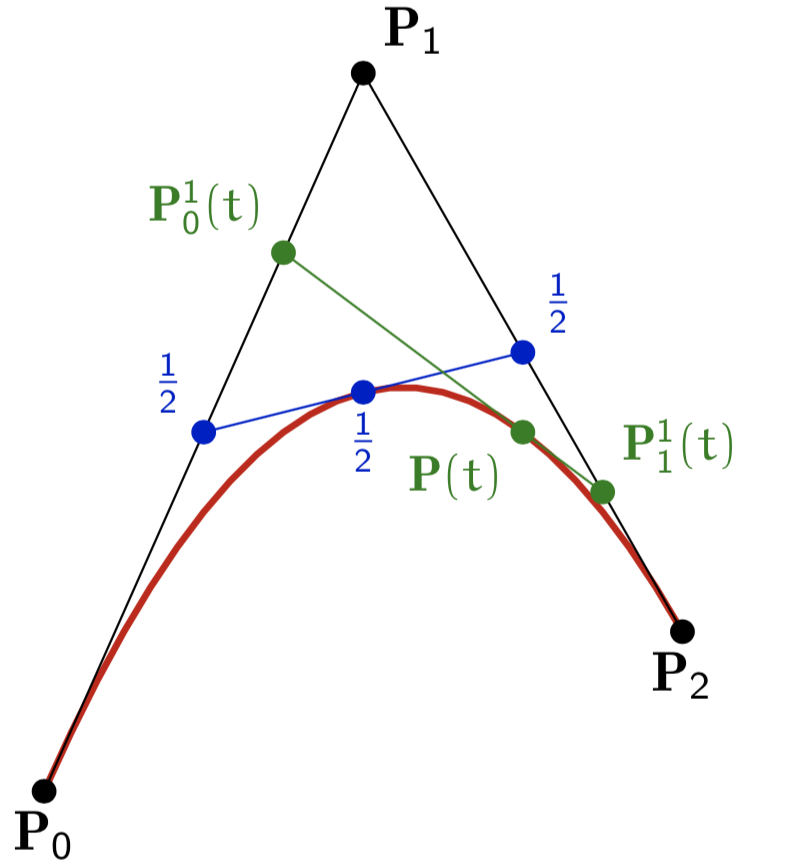
\includegraphics[width=0.3\textwidth]{assets/quadratischeBesierSpline.png}

\textit{drei Kontrollpunkte $P_0, P_1, P_2$}\\

$P_0^1(t) = (1-t)P_0 + P_1$ \\
$P_1^1(t) = (1-t)P_0 + P_1$ \\

$P(t) = (1 - t)^2P_0 + 2(1 - t)tP_1 + t^2 P_2$

\subsection{Qubic Bézier Spline (Approximation)}
\textit{Punkt = Punkt auf Linie zwischen zwei Hilfslinien}\\
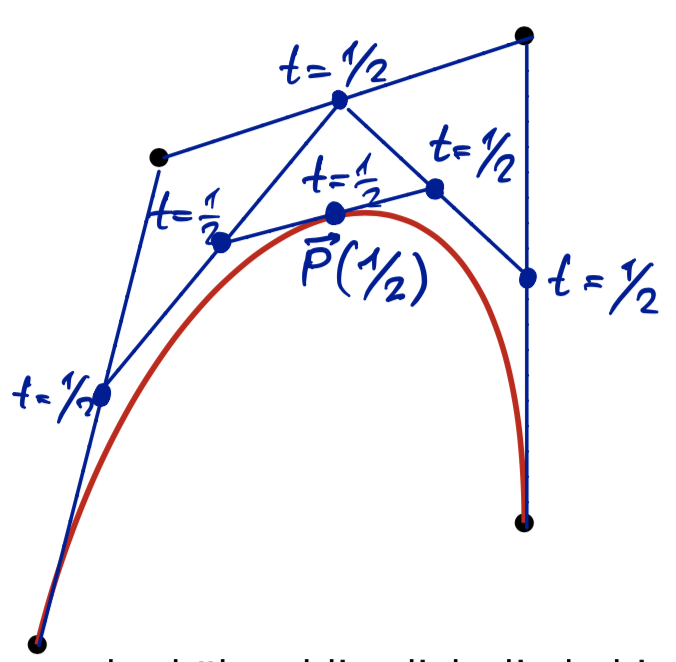
\includegraphics[width=0.3\textwidth]{assets/qubicBesierSpline.png}

\textit{vier Kontrollpunkte $P_0, P_1, P_2, P_3$}\\

\textit{Mit $P_0^1$, $P_1^1$ und} \\
$P_2^1(t) = (1-t)P_2 + tP_3$ \\

$P_1^2(t) = (1 - t) P_0^1(t) + tP_1^1(t)$ \\
$P_2^2(t) = (1 - t) P_1^1(t) + tP_2^1(t)$ \\

$P(t) = (1 - t)^3P_0 + 3(1 - t)^2tP_1 + 3(1 - t)t^2P_2 + t^3P_3$

\subsection{Bernsteinpolynome}

\textit{Bernsteinpolynom für kubische Bézier-Spline:}\\
$B^3_i(t) = \left(\begin{matrix}
    3 \\ i
\end{matrix}\right) (1-t)^{3-i}t^i$, $(0 \leq i \leq 3)$\\

\textit{Dadurch folgt $P(t)$, wobei $P_n$ Kontrollpunkte sind:} \\
$P(t) = (1 - t)^3P_0 + 3(1 - t)^2tP_1 + 3(1 - t)t^2P_2 + t^3P_3 = \displaystyle \sum_{i=0}^{3}( B_i^3(t) P_i )$ \\

\textit{Allgemein bedeutet dies also bei $n$-Anzahl:}\\
$\displaystyle \sum^n_{i=0}(B^n_i(t)P_i)$\\
$B_i^n(t) = \left(\begin{matrix}
    n \\ i
\end{matrix}\right) (1 - t)^{n-i}t^i$, $(0 \leq i \leq n)$\\

\textit{Die Bernoulli Pyramide verhilft beim auflösen:}\\
\[
    \begin{matrix}
          &   &   &   & 1 &   &   &   & \\
          &   &   & 1 &   & 1 &   &   & \\
          &   & 1 &   & 2 &   & 1 &   & \\
          & 1 &   & 3 &   & 3 &   & 1 & \\
        1 &   & 4 &   & 6 &   & 4 &   & 1 \\
      \vdots&&\vdots&&\vdots&&\vdots&&\vdots \\
    \end{matrix}
\]

\subsection{Eigenschaft Bernsteinpolynome}

\begin{itemize}
    \item Die gweichtung addiert sich zu eins: \\
        $B_i^n(t) = \left(\begin{matrix}
            n \\ i
        \end{matrix}\right) (1 - t)^{n-i}t^i = 1^3 = 1$
    \item Die Funktionswerte sind immer grösser gleich Null:\\
        $B_i^n(t) \geq 0$ für $i = 0,1,\dots, n$, $t \in [0,1]$
    \item  $B^i_n(t)$ ist maximal für $t=\frac{i}{n}$, $i = 0,1,\dots, n$
    \item Sind Symetrisch: \\
          $B^n_i(t) = B^n_{n-i}(1-t)$, $i = 0,1,\dots, n$
    \item Rekursiveigenschaft:$B^{n+1}_{i+1}(t) = tB_i^n(t) + (1-t)B^n_{i+1}(t)$
    \item Differation: \\
        $\frac{d}{dt}(B^n_i(t)) = n[B^{n-1}_{i-1}(t) - B^{n-1}_i(t)]$,\\
        $i = 0,1,\dots, (n-1)$\\
        \textit{Beachte bei: $B_{-1}^{n-1}=0$}
\end{itemize}

\subsection{Rekursiveigenschaft Bézier-Kurven}

\textit{Die Rekursiveigenschaft zeigt auf, dass die Bezierkurve in
kleinere Ordnungen aufgeteilt werden kann:}\\

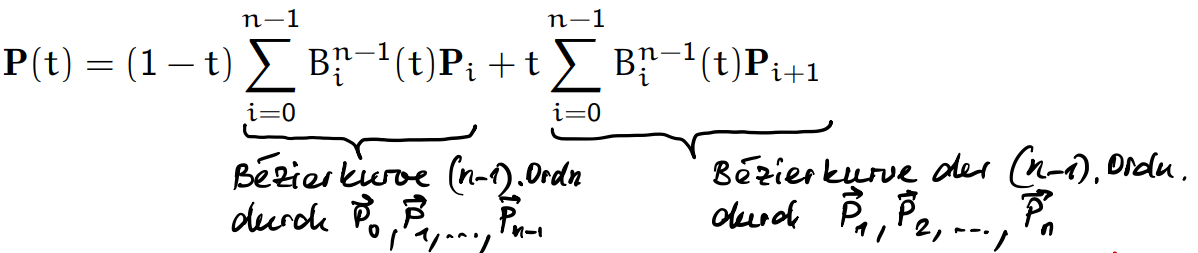
\includegraphics[width=0.5\textwidth]{assets/curves-recursive-spline.png}

\subsection{Bézier-Kurven}

\textbf{Eigenschaften}

\begin{tabular}{cl}
    \multirow{8}{*}{
        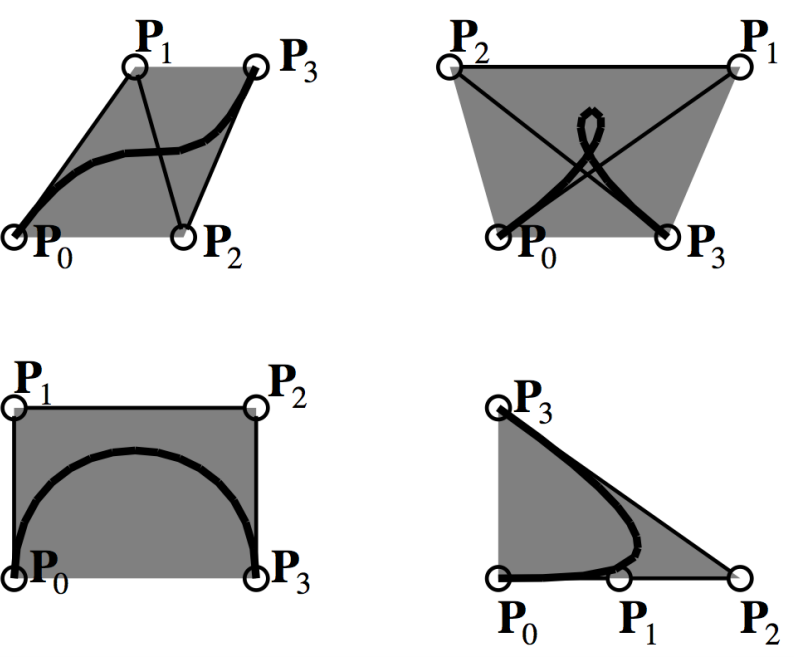
\includegraphics[width=0.19\textwidth]{assets/curves-qubic-besier-curve.png}
    } & \\
    & \\
    & \textit{Die Bézier-Kurve liegt immer}\\
    & \textit{innerhalb der konvexen Hülle}\\
    & \textit{des Linienzuges} \\
    & \textit{(convex hull property)} \\
    & \\
    & \\
\end{tabular}
\begin{itemize}
    \item \textit{Die Anzahl der Kontrollpunkte $P_0, P_1, \dots, P_n$
    bestimmt den Grad n der Bézier-Kurve}\\
    \item \textit{Änderung eines Kontrollpunktes bewirkt eine
    Änderung der gesamten Kurve}\\
    \item \textit{Setzt man stetige Funktionswerte und
    Ableitungen voraus, lassen sich Bézier-Kurven
    höheren Grades durch Bézier-Kurven
    niedrigeren Grades zusammensetzen.}\\
\end{itemize}
\textbf{Stetigkeit}
\begin{itemize}
    \item[$C^0$]-Stetigkeit: Segmente haben an den Eckpunkte keine Sprünge
    \item[$C^1$]-Stetigkeit: Segmente haben an den Eckpunkte gemeinsame Tangente (erste Ableitung gleich)
    \item[$C^2$]-Stetigkeit: Segmente haben an den Eckpunkte die selbe Krümmung (zweite Ableitung gleich)
\end{itemize}

\subsection{B-Spline-Kurven}

\textit{Verallgemeinerung der Bézier-Kurven
(Ordnung kann kleiner als Anzahl Kontrollpunkte sein):}\\

$B_{n,k}(t) = \displaystyle \sum^n_{j=0}(N_{j,k}(t) P_j)$\\

\textit{$k$: Ordnung der Kurve} $2 \leq k \leq n+1$\\
\textit{$t$: gleich wie bei Bézier} $t \in [0, n-k+2]$\\

\textit{$k=2$: linear}\\
\textit{$k=3$: quadtratisch}\\
\textit{$k=4$: kubisch}

\subsection{B-Splines}

\textit{$N_{j,k}(t)$ sind die B-Splines (Gewichtsfunktion, blending functions)}\\
\textit{Sie sind $k$-Ordnung und ($k-1$) Polynome}\\
\textit{Dabei geht es um nichts anders als Bézier-Kurven mit Gewichtung zu verknüpfen,
abhängig der Ordnung wird die Verknüpfung weicher}\\
\textit{Sind Rekursiv definiert}\\

$N_{j,1} = $

\begin{itemize}
	\item lokale Funktionen nur in der Nähe von Pj verschieden von 0
	\item Einfluss vom Punkt auf die gesamte Kurve ist kleiner
\end{itemize}

\subsection{NURBS (Non Uniform Rational Basic Splines)}
TODO
\begin{itemize}
	\item homogenisiert
	\item rationale B-Spline-Kurve
	\item Punkte mit Gewichtung
	\item invariant bei den Transformationen
\end{itemize}